% ============================================================
%  Adversarial Robustness in VIPGuard — Conference Paper
%  Single-column, 10-12 pages
%  Compile: pdflatex vipguard_conference_paper.tex  (run twice)
% ============================================================
\documentclass[12pt,a4paper]{article}

\usepackage[margin=2.5cm]{geometry}
\usepackage{amsmath,amssymb}
\usepackage{graphicx}
\usepackage{booktabs}
\usepackage{array}
\usepackage{xcolor}
\usepackage{hyperref}
\usepackage{cite}
\usepackage{caption}
\usepackage{float}
\usepackage{enumitem}
\usepackage{parskip}
\usepackage{fancyhdr}
\usepackage{titlesec}
\usepackage{microtype}
\usepackage{multirow}
\usepackage{tabularx}
\usepackage{listings}
\usepackage{setspace}

% ── Colours ───────────────────────────────────────────────────────────────────
\definecolor{deepblue}{RGB}{0,70,140}
\definecolor{codegreen}{RGB}{0,128,64}
\definecolor{codegray}{RGB}{128,128,128}
\definecolor{codepurple}{RGB}{128,0,128}
\definecolor{codebackground}{RGB}{248,248,248}

% ── Hyperref ──────────────────────────────────────────────────────────────────
\hypersetup{
  colorlinks=true, linkcolor=deepblue,
  citecolor=deepblue, urlcolor=deepblue,
  pdftitle={Adversarial Robustness in VIPGuard},
}

% ── Section formatting ────────────────────────────────────────────────────────
\titleformat{\section}{\large\bfseries\color{deepblue}}{\thesection.}{0.6em}{}
\titleformat{\subsection}{\normalsize\bfseries\color{deepblue}}{\thesubsection.}{0.6em}{}
\titleformat{\subsubsection}{\normalsize\bfseries}{\thesubsubsection.}{0.6em}{}

% ── Header / footer ───────────────────────────────────────────────────────────
\pagestyle{fancy}
\fancyhf{}
\rhead{\small\textit{Adversarial Robustness in VIPGuard}}
\lhead{\small\textit{Conference Paper --- 2026}}
\cfoot{\thepage}
\renewcommand{\headrulewidth}{0.4pt}

% ── Code style ────────────────────────────────────────────────────────────────
\lstset{
  language=Python,
  backgroundcolor=\color{codebackground},
  basicstyle=\ttfamily\footnotesize,
  keywordstyle=\color{deepblue}\bfseries,
  commentstyle=\color{codegreen}\itshape,
  stringstyle=\color{codepurple},
  numbers=left, numberstyle=\tiny\color{codegray}, numbersep=6pt,
  breaklines=true, frame=single, rulecolor=\color{codegray},
  tabsize=4, showstringspaces=false,
  xleftmargin=12pt, xrightmargin=4pt,
  aboveskip=6pt, belowskip=6pt,
}

% ── Utility macros ────────────────────────────────────────────────────────────
\newcommand{\norm}[1]{\left\lVert#1\right\rVert}
\newcommand{\sign}{\operatorname{sign}}
\newcommand{\E}{\mathbb{E}}

% ══════════════════════════════════════════════════════════════════════════════
\begin{document}
% ══════════════════════════════════════════════════════════════════════════════

% ── Title block ───────────────────────────────────────────────────────────────
\begin{center}
{\LARGE\bfseries\color{deepblue}
  Adversarial Robustness of VIPGuard:\\[4pt]
  Defending VIP Identity Verification Against\\[4pt]
  Adversarial Attacks via Curriculum Training
}

\vspace{14pt}
{\large Anonymous Author(s)}\\[4pt]
{\normalsize Institution Withheld for Review}\\[4pt]
{\small \texttt{anonymous@institution.edu}}

\vspace{10pt}
\rule{0.5\textwidth}{0.4pt}
\end{center}

% ══════════════════════════════════════════════════════════════════════════════
\begin{abstract}
% ══════════════════════════════════════════════════════════════════════════════

VIPGuard is a Vision-Language Model (VLM) based system that combines the
32-billion parameter Qwen2.5-VL with learned per-VIP token embeddings to
simultaneously verify the identity of registered VIP individuals and detect
deepfake manipulations.  While VIPGuard achieves near-perfect accuracy on clean
images, we show for the first time that it is completely vulnerable to white-box
adversarial attacks that target the underlying TransFace face embedding model.
A simple Fast Gradient Sign Method (FGSM) attack with $\varepsilon = 8/255$
reduces the face similarity score from $\sim\!91/100$ to $47$--$75/100$,
causing the model to reject authentic VIP images with 100\% failure rate.
Stronger Projected Gradient Descent (PGD) attacks reduce the score further to
$13$--$34/100$ with identical failure rates.

To restore robustness, we design and implement a two-stage curriculum adversarial
training strategy.  In Stage~1, VIP tokens are initialised from scratch and
trained on clean data at high learning rate ($\eta = 1.0$) to build visual
discrimination capability.  In Stage~2, training continues from the Stage~1
checkpoint at a reduced learning rate ($\eta = 0.1$) on a dataset mixing 85\%
clean and 15\% adversarially perturbed examples, using post-attack similarity
scores in prompts to match the evaluation distribution.  This curriculum fully
solves PGD robustness (0\% $\to$ 100\% across all tested identities) while
preserving normal-real authentication (100\%) and achieving partial FGSM
robustness.  We provide a complete experimental analysis of five training
strategies, documenting why each fails or succeeds, and identify the fundamental
challenge: the similarity-score overlap between FGSM-perturbed real images
(46--75/100) and deepfakes (52--86/100) that makes simultaneous robustness and
deepfake detection difficult to achieve with a single policy.

\end{abstract}

\vspace{6pt}
\noindent\textbf{Keywords:} adversarial robustness, face verification, deepfake
detection, FGSM, PGD, vision-language model, curriculum adversarial training,
VIPGuard.

\newpage

% ══════════════════════════════════════════════════════════════════════════════
\section{Introduction}
% ══════════════════════════════════════════════════════════════════════════════

The proliferation of sophisticated deepfake generation techniques~\cite{rossler2019faceforensics,li2020celeb} has made
automated face verification increasingly difficult.  Face-swapping algorithms,
generative adversarial networks, and diffusion-based synthesis can produce
photorealistic images that are indistinguishable to the human eye, posing serious
threats to identity verification systems used in access control, financial
authentication, and security screening.

At the same time, adversarial attacks on face recognition models present a
complementary and equally serious threat.  An attacker who adds carefully crafted,
visually imperceptible noise to a genuine photograph can cause state-of-the-art
face embedding models to assign it a near-zero similarity score, effectively
making the legitimate VIP appear to be an impostor~\cite{goodfellow2014explaining,madry2018towards}.

VIPGuard~\cite{vipguard2024} addresses the deepfake detection side of this
problem using a novel approach: rather than training a standalone binary
classifier, it injects per-VIP learned token embeddings into a frozen
32-billion-parameter Vision-Language Model (Qwen2.5-VL~\cite{bai2025qwen2vl}),
enabling the model to reason about identity in natural language.  VIPGuard
achieves near-perfect accuracy on clean images and deepfakes.

\textbf{The gap we address.} VIPGuard was not designed or evaluated under
adversarial attack conditions.  This paper is the first systematic study of
VIPGuard's adversarial vulnerability and the first attempt to restore robustness
through adversarial training.

\subsection*{Contributions}

We make the following contributions:

\begin{enumerate}[leftmargin=*]
  \item \textbf{Adversarial vulnerability analysis.}  We demonstrate that VIPGuard
  has 0\% accuracy under FGSM and PGD attacks targeting the TransFace face embedding
  model, even though the VLM itself is not attacked.

  \item \textbf{Attack implementation.}  We implement FGSM and PGD attacks against
  TransFace, handling the \texttt{@torch.no\_grad()} barrier and autocast gradient
  underflow pitfalls that arise in the production inference pipeline.

  \item \textbf{Adversarial dataset generation.}  We generate a dataset of
  adversarially perturbed probe images for three VIP identities (id0, id1, id2),
  each paired with post-attack similarity scores used in training prompts.

  \item \textbf{Systematic training ablation.}  We run five distinct training
  strategies (R0--R4), documenting the root cause of each failure and deriving
  the design of the curriculum approach.

  \item \textbf{Curriculum adversarial training (R5).}  Our two-stage curriculum
  achieves 100\% PGD robustness on all identities while maintaining 100\% accuracy
  on clean real images.
\end{enumerate}

% ══════════════════════════════════════════════════════════════════════════════
\section{Related Work}
% ══════════════════════════════════════════════════════════════════════════════

\subsection{Deepfake Detection}

Early deepfake detectors used handcrafted features such as eye blinking patterns
and facial landmark inconsistencies~\cite{li2018ictu}.  More recent approaches
use convolutional neural networks trained on FaceForensics++~\cite{rossler2019faceforensics},
a benchmark covering four manipulation methods.  CelebDF~\cite{li2020celeb} and
DFDC~\cite{dolhansky2020deepfake} provide larger-scale benchmarks.  These
detectors are binary classifiers and do not provide natural-language reasoning.

\subsection{Vision-Language Models for Face Analysis}

Large Vision-Language Models such as GPT-4V and Qwen2.5-VL~\cite{bai2025qwen2vl} have
demonstrated strong zero-shot visual reasoning.  VIPGuard~\cite{vipguard2024}
exploits this by adding a lightweight learnable interface---the FaceChecker---that
adapts the frozen VLM to per-VIP identity verification without retraining the
32B backbone.

\subsection{Adversarial Attacks on Face Recognition}

Goodfellow et al.~\cite{goodfellow2014explaining} introduced the Fast Gradient Sign
Method (FGSM), a single-step attack that perturbs the input in the direction of
the loss gradient.  Madry et al.~\cite{madry2018towards} extended this to
Projected Gradient Descent (PGD), a multi-step attack that is widely considered
the strongest first-order attack.  Face-specific adversarial attacks have targeted
ArcFace~\cite{deng2019arcface} and CosFace, typically aiming to dodge recognition
by maximising the angle between the adversarial embedding and the enrollment
centre.

\subsection{Adversarial Training}

Madry et al.~\cite{madry2018towards} showed that training on PGD adversarial
examples yields models certifiably robust under PGD attacks.  Trades~\cite{zhang2019theoretically}
established a formal trade-off between accuracy and robustness.  These methods
train the full model; our setting is different because the 32B VLM is frozen and
only the small VIP token embeddings (114,688 parameters) are trainable, making
adversarial training significantly more constrained.

% ══════════════════════════════════════════════════════════════════════════════
\section{Original VIPGuard Framework}
% ══════════════════════════════════════════════════════════════════════════════

\subsection{System Overview}

VIPGuard performs two tasks jointly: \emph{VIP identity verification} (is the
person in the image the registered VIP?) and \emph{deepfake detection} (is the
image authentic or synthetically generated?).  Both tasks are framed as a
single yes/no question answered by a frozen 32B VLM.

The system comprises four main components:

\begin{enumerate}[leftmargin=*]
  \item \textbf{TransFace} --- a Vision Transformer (ViT-L) face embedding model
  that maps a $112\times112$ RGB image to a 512-dimensional $\ell_2$-normalised
  embedding.

  \item \textbf{Face Embedding Centre} --- a per-VIP reference embedding $\mathbf{c}_k$
  precomputed from multiple enrolment images of VIP identity~$k$.

  \item \textbf{FaceChecker} --- a CrossAttention module that maps learnable VIP
  prompt tokens $\mathbf{P}_k \in \mathbb{R}^{N \times 3584}$ and image features
  from the VLM vision encoder into face embedding tokens that replace the
  \texttt{<|face\_pad|>} special token positions in the LLM input.

  \item \textbf{Qwen2.5-VL} --- a frozen 32-billion-parameter Vision-Language
  Model that processes the combined face embedding tokens, image tokens, and text
  tokens to generate a verdict.
\end{enumerate}

\subsection{Inference Pipeline}

\subsubsection{Step 1: Similarity Scoring}

Given a probe image $x$, TransFace produces an embedding
$\mathbf{e} = f_{\text{TF}}(x) \in \mathbb{R}^{512}$.  The similarity score is

\begin{equation}
  s = \left\lfloor \left( 0.5 + 0.5 \cdot
  \frac{\mathbf{e} \cdot \mathbf{c}_k}{\norm{\mathbf{e}}\norm{\mathbf{c}_k}}
  \right) \times 100 \right\rfloor \in [0, 100].
  \label{eq:sim}
\end{equation}

This maps cosine similarity $[-1, 1]$ linearly to an integer score in $[0, 100]$.
The score is embedded as text in the user prompt: \emph{``Similarity $s$/100.
Is this VIP person?''}.

\subsubsection{Step 2: VIP Token Injection}

The learnable VIP prompt $\mathbf{P}_k$ encodes identity-specific visual
information for VIP~$k$.  The FaceChecker performs multi-head cross-attention:

\begin{equation}
  \mathbf{F} = \text{CrossAttention}(\,Q = \phi(x),\ K = V = \mathbf{P}_k\,),
  \label{eq:facechecker}
\end{equation}

where $\phi(x)$ denotes the image features from the Qwen2.5-VL vision encoder.
The resulting face embedding tokens $\mathbf{F}$ replace the
\texttt{<|face\_pad|>} positions in the token sequence fed to the LLM.

\subsubsection{Step 3: VLM Generation}

The LLM autoregressively generates a response in the format:

\begin{center}
\texttt{<Conclusion>[Yes/No] \ldots natural-language reasoning \ldots</Conclusion>}
\end{center}

The frozen LLM uses both the similarity score text signal and the visual face
embedding tokens to produce its decision.

\subsection{Training Protocol}

VIP tokens are trained in Stage~3 of the original VIPGuard pipeline.  The 32B
LLM is fully frozen; only $\mathbf{P}_k$ (shape $[32, 3584]$, totalling
114,688 parameters) is updated via AdamW with a cosine learning rate schedule.
Loss is computed only on assistant-role tokens (question tokens are masked with
$-100$).  A separate $\mathbf{P}_k$ is trained per VIP identity.

% ══════════════════════════════════════════════════════════════════════════════
\section{Proposed Adversarial Extension}
% ══════════════════════════════════════════════════════════════════════════════

\subsection{Threat Model}

We consider a \emph{white-box dodge attacker} who:
(i) has full access to the TransFace model and its weights,
(ii) is limited to additive $\ell_\infty$ perturbations of magnitude
     $\varepsilon = 8/255$ in pixel space (visually imperceptible),
(iii) aims to make a genuine VIP image be rejected (\emph{dodging}),
(iv) does \emph{not} have access to the VLM weights or VIP tokens.

The attack targets TransFace because: (a) it provides the similarity score that
acts as a strong prior in the VLM prompt, and (b) computing gradients through a
32B model would be prohibitively expensive.

\subsection{Image Normalisation Convention}

TransFace operates on images normalised to $[-1, 1]$ via:

\begin{equation}
  \tilde{x} = \frac{x_{\text{pixel}} / 255 - 0.5}{0.5},
\end{equation}

where $x_{\text{pixel}} \in [0, 255]$.  An $\ell_\infty$ perturbation of
$\varepsilon = 8/255$ in pixel space corresponds to
$\varepsilon_n = \varepsilon / 0.5 \approx 0.0627$ in normalised space.

\subsection{FGSM Attack}
\label{sec:fgsm}

The Fast Gradient Sign Method~\cite{goodfellow2014explaining} computes a
single gradient step.  Our objective is to \emph{minimise} the cosine similarity
between the adversarial embedding and the VIP centre $\mathbf{c}_k$:

\begin{equation}
  \mathcal{L}_{\text{adv}}(\tilde{x}) =
  \frac{f_{\text{TF}}(\tilde{x})}{\norm{f_{\text{TF}}(\tilde{x})}}
  \cdot \hat{\mathbf{c}}_k,
  \quad
  \hat{\mathbf{c}}_k = \frac{\mathbf{c}_k}{\norm{\mathbf{c}_k}}.
  \label{eq:advloss}
\end{equation}

The adversarial image is:

\begin{equation}
  \tilde{x}_{\text{adv}} =
  \Pi_{[-1,1]}\!\left(
    \tilde{x} + \varepsilon_n \cdot \sign\!\left(\nabla_{\tilde{x}}\,
    \mathcal{L}_{\text{adv}}(\tilde{x})\right)
  \right),
  \label{eq:fgsm}
\end{equation}

where $\Pi_{[-1,1]}$ clips all values to $[-1,1]$ to satisfy the valid image
range constraint.  Note the \emph{positive} gradient direction: we maximise the
loss (i.e., move the embedding away from the centre).

\subsubsection*{Implementation pitfalls}

Two non-obvious implementation issues arise in the VIPGuard codebase:

\begin{enumerate}[leftmargin=*]
  \item \textbf{\texttt{@torch.no\_grad()} barrier.}  The production method
  \texttt{FG\_Face.face\_emb\_forward()} is decorated with
  \texttt{@torch.no\_grad()}, which silently returns zero gradients.  The attack
  must call the raw ViT backbone \texttt{face\_model.face\_model(x)} directly,
  which returns a 3-tuple \texttt{(feat, weight, patch\_entropy)}.

  \item \textbf{Autocast gradient underflow.}  The TransFace attention layers use
  \texttt{torch.cuda.amp.autocast(True)} internally.  FP16 arithmetic can cause
  gradient underflow in the attack's backward pass, producing zero gradients.
  The fix is to wrap the forward pass in
  \texttt{torch.amp.autocast('cuda', enabled=False)}, forcing FP32 for the
  attack computation.
\end{enumerate}

\subsection{PGD Attack}
\label{sec:pgd}

Projected Gradient Descent~\cite{madry2018towards} applies FGSM iteratively
with step size $\alpha = 2/255$, projecting back into the $\varepsilon$-ball
after each step.  Let $\tilde{x}^{(0)} = \tilde{x} + \delta_0$ where
$\delta_0 \sim \mathcal{U}[-\varepsilon_n, \varepsilon_n]^d$ (random start).
Then for $t = 1, \ldots, T$:

\begin{align}
  \tilde{x}^{(t)} &=
  \Pi_{B_{\varepsilon_n}(\tilde{x})}\!\left(
    \tilde{x}^{(t-1)}
    + \alpha_n \cdot \sign\!\left(
      \nabla_{\tilde{x}^{(t-1)}} \mathcal{L}_{\text{adv}}(\tilde{x}^{(t-1)})
    \right)
  \right), \label{eq:pgd}
\end{align}

where $\Pi_{B_{\varepsilon_n}(\tilde{x})}$ denotes projection onto the
$\ell_\infty$ ball of radius $\varepsilon_n$ centred at $\tilde{x}$, i.e.,

\begin{equation}
  \delta = \tilde{x}^{(t)} - \tilde{x}, \quad
  \delta \leftarrow \operatorname{clip}(\delta, -\varepsilon_n, \varepsilon_n), \quad
  \tilde{x}^{(t)} = \operatorname{clip}(\tilde{x} + \delta, -1, 1).
  \label{eq:projection}
\end{equation}

We use $T = 10$ steps.  A critical implementation detail: at each step,
$\tilde{x}^{(t-1)}$ must be detached from the computation graph
(\texttt{.detach().requires\_grad\_(True)}) before recomputing gradients,
otherwise PyTorch retains the entire unrolled graph in memory and the process
runs out of GPU memory.

\subsubsection*{FGSM vs PGD}

Table~\ref{tab:attackcomp} summarises the key differences.

\begin{table}[H]
\centering
\caption{Comparison of FGSM and PGD attacks}
\label{tab:attackcomp}
\begin{tabular}{@{}lll@{}}
\toprule
\textbf{Property}       & \textbf{FGSM} & \textbf{PGD ($T=10$)} \\
\midrule
Steps                   & 1             & 10 \\
Step size               & $\varepsilon$ & $\alpha = \varepsilon/4$ \\
Random start            & No            & Yes \\
Attack strength         & Weak          & Strong \\
Sim score (mean, id0)   & 63.5/100      & 23.6/100 \\
Baseline accuracy drop  & $-100\%$      & $-100\%$ \\
\bottomrule
\end{tabular}
\end{table}

Both attacks achieve 100\% failure rate at baseline because the similarity
score drop is sufficient to trigger rejection even for FGSM (score drops from
$\sim\!91$ to $47$--$75$, which the model interprets as a non-VIP).

\subsection{Adversarial Dataset Generation}

For each VIP identity $k \in \{0,1,2\}$, we apply both FGSM and PGD to all
probe images from the \texttt{r\_r\_i} (real same-identity) category.  We store:

\begin{itemize}[leftmargin=*]
  \item \texttt{data/adversarial/\{fgsm,pgd\}/adv\_real/id\{k\}/id\{k\}\_\{n\}/adv.png}
        --- the adversarial image,
  \item \texttt{sim.txt} --- the post-attack similarity score $s_{\text{adv}}$
        (Equation~\ref{eq:sim} applied to $\tilde{x}_{\text{adv}}$),
  \item \texttt{orig\_sim.txt} --- the pre-attack score $s_{\text{orig}}$.
\end{itemize}

A JSON training file is constructed per identity by mixing the original Stage~3
clean training JSON with adversarial entries.  Each adversarial entry uses the
post-attack similarity score $s_{\text{adv}}$ in its prompt and carries the
authentic-VIP label (\texttt{[Yes]}).  This is critical: using the pre-attack
score $s_{\text{orig}}$ in adversarial training prompts creates a
train/evaluation distribution mismatch that causes 100\% FGSM/PGD failure at
evaluation time (documented as Run~R3, Section~\ref{sec:results}).

% ══════════════════════════════════════════════════════════════════════════════
\section{Robustness Evaluation Framework}
% ══════════════════════════════════════════════════════════════════════════════

\subsection{Evaluation Categories}

For each VIP identity we construct four evaluation sets of 30 images each:

\begin{enumerate}[leftmargin=*]
  \item \textbf{normal\_real} --- clean, unperturbed probe images from
        \texttt{r\_r\_i}. True label: \emph{Yes} (authentic VIP).
  \item \textbf{deepfake} --- face-swapped (\texttt{r\_fs\_i}) and
        entire-face-synthesised (\texttt{r\_efs\_i}) images.
        True label: \emph{No}.
  \item \textbf{fgsm\_attack} --- FGSM-perturbed probe images.
        True label: \emph{Yes} (same person, just perturbed).
  \item \textbf{pgd\_attack} --- PGD-perturbed probe images.
        True label: \emph{Yes}.
\end{enumerate}

\subsection{Metrics}

Let $N$ denote the total number of samples and define:
TP (model says Yes; truth is Yes),
TN (No; No), FP (Yes; No), FN (No; Yes).

\begin{align}
  \text{Accuracy} &= \frac{\text{TP} + \text{TN}}{N}, \label{eq:acc} \\[4pt]
  \text{FAR} &= \frac{\text{FP}}{\text{FP} + \text{TN}}, \label{eq:far} \\[4pt]
  \text{FRR} &= \frac{\text{FN}}{\text{FN} + \text{TP}}, \label{eq:frr} \\[4pt]
  \Delta\text{Acc} &= \frac{\text{Acc}_{\text{normal}} - \text{Acc}_{\text{adv}}}{\text{Acc}_{\text{normal}}} \times 100\%. \label{eq:drop}
\end{align}

FAR (False Acceptance Rate) is relevant for deepfake categories: it measures
the fraction of impostor images incorrectly authenticated as the VIP, which is
the most security-critical failure mode.  FRR (False Rejection Rate) applies to
authentic and adversarial-real categories: it measures how often a legitimate VIP
is rejected.  Performance drop $\Delta\text{Acc}$ quantifies degradation from
clean to adversarial conditions.

\subsection{Similarity Score Distribution}

Figure~\ref{fig:simdist} illustrates the similarity score distributions for id0.
The non-overlapping region between normal\_real ($79$--$95/100$) and PGD
($13$--$34/100$) is large; however, FGSM ($46$--$75/100$) and deepfake
($52$--$78/100$) overlap almost entirely, which is the fundamental challenge
addressed by our work.

\begin{figure}[H]
\centering
\includegraphics[width=0.85\textwidth]{../results/before_adv_train/id0_sim_distribution.png}
\caption{Similarity score distributions for id0 before adversarial training.
         The FGSM and deepfake distributions almost completely overlap in the
         range $47$--$75/100$, preventing the model from using the text similarity
         signal alone to distinguish a perturbed real face from a deepfake.}
\label{fig:simdist}
\end{figure}

% ══════════════════════════════════════════════════════════════════════════════
\section{Adversarial Training}
% ══════════════════════════════════════════════════════════════════════════════

\subsection{Training Setup}

All training updates only the VIP prompt $\mathbf{P}_k \in \mathbb{R}^{32 \times 3584}$
via AdamW.  The 32B VLM is frozen throughout.  Gradient accumulation over
8 steps with \texttt{bf16} mixed precision is used to handle the large model
on a single 24~GB GPU.  Loss is causal LM cross-entropy restricted to
assistant-role tokens.

\subsection{Experimental Design: Five Training Strategies}
\label{sec:training_strategies}

Table~\ref{tab:rundesign} summarises the five strategies we evaluated.

\begin{table}[H]
\centering
\caption{Training strategy design for all experimental runs}
\label{tab:rundesign}
\begin{tabular}{@{}p{1.6cm}p{1.8cm}p{1.0cm}p{1.0cm}p{1.2cm}p{4.5cm}@{}}
\toprule
\textbf{Run} & \textbf{Token Init} & \textbf{LR} & \textbf{Ep.} & \textbf{Adv\%} & \textbf{Key Design Choice} \\
\midrule
R0 Baseline & pretrained & --- & --- & 0   & No adversarial training \\
R1          & pretrained & 0.001 & 3 & 25 & Short prompt format (mismatch with eval) \\
R2          & pretrained & 1.0   & 3 & 25 & Correct prompt, high LR on pretrained tokens \\
R3          & scratch    & 1.0   & 5 & 50 & \texttt{orig\_sim} in prompts (train/eval mismatch) \\
R4          & scratch    & 1.0   & 5 & 50 & \texttt{adv\_sim} in prompts, no curriculum \\
R5 (ours)   & scratch    & 1.0 / 0.1 & 3+3 & 0 / 15 & Two-stage curriculum \\
\bottomrule
\end{tabular}
\end{table}

\subsection{The Two-Stage Curriculum (R5)}

\subsubsection*{Motivation}

Runs R3 and R4 reveal the core dilemma:

\begin{itemize}[leftmargin=*]
  \item Using \emph{high} similarity scores in adversarial training prompts
  (R3: \texttt{orig\_sim} $\approx 91/100$) produces a train/eval mismatch ---
  at evaluation time the perturbed images have scores of $47$--$75$, which
  the trained tokens have never seen, so the model rejects them.

  \item Using \emph{low} similarity scores in adversarial training prompts
  (R4: \texttt{adv\_sim} $\approx 47$--$75$) matches the evaluation distribution
  and achieves 100\% FGSM/PGD robustness, but the model learns \emph{``accept
  images with sim 47--75''}.  Deepfakes for some identities also have sim
  $52$--$78$, so the model accepts them too, collapsing deepfake detection to
  near zero.
\end{itemize}

The root cause is that FGSM attacks target TransFace, \emph{not} Qwen2.5-VL.
The VLM's vision encoder still sees a genuine face with imperceptible noise;
its visual features are nearly identical to those of the clean image.  Therefore,
VIP tokens can in principle learn to trust the visual signal even when the text
similarity score is low --- but only if they first establish a strong visual
model of identity and deepfake characteristics.

\subsubsection*{Stage~1: Visual Foundation (Clean, LR = 1.0, 3 epochs)}

VIP tokens are initialised randomly (\texttt{nn.init.normal\_}) and trained on
the original clean Stage~3 JSON.  This stage teaches:

\begin{enumerate}[leftmargin=*]
  \item Authenticate real VIP images based on visual features.
  \item Reject deepfakes using visual feature discrepancies, not just the
        similarity score text signal.
\end{enumerate}

High learning rate ($\eta = 1.0$) accelerates learning from random initialisation.

\subsubsection*{Stage~2: Adversarial Fine-tuning (Mixed, LR = 0.1, 3 epochs, adv = 15\%)}

Starting from the Stage~1 checkpoint, training continues with a dataset composed
of 85\% original clean examples and 15\% adversarial examples.  Adversarial
prompts use \texttt{adv\_sim} to match the evaluation distribution.

The 10$\times$ lower learning rate ($\eta = 0.1$) serves two purposes:
(i) it preserves the visual discrimination learned in Stage~1, and
(ii) it introduces adversarial robustness gently, preventing the token from
over-fitting to the \emph{``accept low sim''} heuristic.

The 15\% adversarial fraction (vs.\ 50\% in R4) is another critical difference:
a smaller adversarial fraction exerts less pressure toward the \emph{``accept
medium sim''} policy, allowing the model to maintain deepfake discrimination
for identities where deepfake sim scores are sufficiently distinct.

% ══════════════════════════════════════════════════════════════════════════════
\section{Results and Analysis}
% ══════════════════════════════════════════════════════════════════════════════
\label{sec:results}

\subsection{Baseline Vulnerability (R0)}

Table~\ref{tab:r0} confirms the motivation for this work.  Pretrained VIPGuard
tokens achieve near-perfect accuracy on clean images and deepfakes but fail
completely under adversarial attack.  The model's reliance on the text similarity
score is the key vulnerability: FGSM reduces the score from $\sim\!91$ to
$47$--$75$, which the model interprets as insufficient for authentication.

\begin{table}[H]
\centering
\caption{R0 Baseline results (pretrained tokens, no adversarial training)}
\label{tab:r0}
\begin{tabular}{@{}llcccc@{}}
\toprule
\textbf{ID} & \textbf{Category} & \textbf{Accuracy} & \textbf{FAR/FRR} & \textbf{Sim Mean} \\
\midrule
id0 & normal\_real  & 100.0\% & FRR 0.0\%  & 90.6 \\
id0 & deepfake      &  96.7\% & FAR 3.3\%  & 62.5 \\
id0 & fgsm\_attack  &   0.0\% & FRR 100\%  & 63.5 \\
id0 & pgd\_attack   &   0.0\% & FRR 100\%  & 23.6 \\
\midrule
id1 & normal\_real  & 100.0\% & FRR 0.0\%  & 93.7 \\
id1 & deepfake      & 100.0\% & FAR 0.0\%  & 64.2 \\
id1 & fgsm\_attack  &   0.0\% & FRR 100\%  & 60.2 \\
id1 & pgd\_attack   &   0.0\% & FRR 100\%  & 19.5 \\
\midrule
id2 & normal\_real  & 100.0\% & FRR 0.0\%  & 92.1 \\
id2 & deepfake      &  80.0\% & FAR 20.0\% & 71.4 \\
id2 & fgsm\_attack  &   0.0\% & FRR 100\%  & 57.7 \\
id2 & pgd\_attack   &   0.0\% & FRR 100\%  & 18.7 \\
\bottomrule
\end{tabular}
\end{table}

\subsection{Intermediate Runs (R1--R4)}

Table~\ref{tab:rall} presents the id0 results for each training strategy.

\begin{table}[H]
\centering
\caption{Training strategy comparison on id0 (30 samples per category)}
\label{tab:rall}
\begin{tabular}{@{}lcccc@{}}
\toprule
\textbf{Run} & \textbf{Normal Real} & \textbf{Deepfake} & \textbf{FGSM} & \textbf{PGD} \\
\midrule
R0 Baseline (no adv. training)     & 100.0\% & 96.7\%  &  0.0\% &  0.0\% \\
R1 Wrong prompt format              & 100.0\% & 95.0\%  &  0.0\% &  0.0\% \\
R2 Pretrained + LR=1.0              &  90.0\% & 95.0\%  &  0.0\% &  0.0\% \\
R3 Scratch + orig\_sim              &  86.7\% & 100.0\% &  0.0\% &  0.0\% \\
R4 Scratch + adv\_sim               & 100.0\% & 26.7\%  & 100.0\% & 100.0\% \\
\textbf{R5 Curriculum (ours)}       & \textbf{100.0\%} & \textbf{96.7\%} & \textbf{46.7\%} & \textbf{100.0\%} \\
\bottomrule
\end{tabular}
\end{table}

\textbf{R1 --- Wrong prompt.}  Training used a short prompt format (\emph{``say yes
or no''}) while evaluation used the long attribute-reasoning format.  The
distribution mismatch meant every gradient step was wasted; token norm change
was $0.019$ over three full epochs, essentially zero learning.

\textbf{R2 --- High LR on pretrained tokens.}  Correcting the prompt, but applying
LR=$1.0$ to pretrained tokens caused catastrophic forgetting of the clean-data
distribution, reducing normal\_real accuracy from $100\%$ to $90\%$.  FGSM/PGD
remained at $0\%$, confirming that fine-tuning pretrained tokens is insufficient.

\textbf{R3 --- Scratch + orig\_sim.}  Training from random initialisation with high
LR avoided forgetting and achieved strong deepfake detection.  However,
adversarial training prompts used $s_{\text{orig}} \approx 91/100$ while
evaluation presents $s_{\text{adv}} \approx 47$--$75/100$.  The tokens learned
the decision boundary \emph{``high sim + VIP tokens $\Rightarrow$ Yes''} ---
completely inapplicable at evaluation time.

\textbf{R4 --- Scratch + adv\_sim.}  Switching to post-attack similarity scores
in training prompts fixed the train/eval mismatch.  FGSM and PGD reached
$100\%$, confirming the hypothesis.  However, deepfake detection collapsed to
$26.7\%$ on id0 and $0\%$ on id2.  With 50\% adversarial fraction and
\emph{``adv\_sim $\approx$ deepfake sim''} overlap, the model learned a blanket
\emph{``accept medium sim''} policy that admitted deepfakes.

\subsection{Curriculum Training Results (R5)}

Table~\ref{tab:r5} presents the full per-identity results for our proposed
curriculum.

\begin{table}[H]
\centering
\caption{R5 Curriculum results: Stage1 (LR=1.0, ep=3, clean) + Stage2 (LR=0.1, ep=3, adv=15\%)}
\label{tab:r5}
\begin{tabular}{@{}llccccc@{}}
\toprule
\textbf{ID} & \textbf{Category} & \textbf{Accuracy} & \textbf{FAR} & \textbf{FRR} & \textbf{Sim Mean} & \textbf{vs.\ R0} \\
\midrule
id0 & normal\_real  & 100.0\% & ---    & 0.0\%  & 90.6 & $\pm 0$      \\
id0 & deepfake      &  96.7\% & 3.3\%  & ---    & 62.5 & $\pm 0$      \\
id0 & fgsm\_attack  &  46.7\% & ---    & 53.3\% & 63.5 & $+46.7$pp   \\
id0 & pgd\_attack   & 100.0\% & ---    & 0.0\%  & 23.6 & $+100$pp    \\
\midrule
id1 & normal\_real  & 100.0\% & ---    & 0.0\%  & 93.7 & $\pm 0$      \\
id1 & deepfake      &  80.0\% & 20.0\% & ---    & 64.2 & $-20$pp     \\
id1 & fgsm\_attack  &  13.3\% & ---    & 86.7\% & 60.2 & $+13.3$pp   \\
id1 & pgd\_attack   & 100.0\% & ---    & 0.0\%  & 19.5 & $+100$pp    \\
\midrule
id2 & normal\_real  & 100.0\% & ---    & 0.0\%  & 92.1 & $\pm 0$      \\
id2 & deepfake      &  43.3\% & 56.7\% & ---    & 71.4 & $-36.7$pp   \\
id2 & fgsm\_attack  & 100.0\% & ---    & 0.0\%  & 57.7 & $+100$pp    \\
id2 & pgd\_attack   & 100.0\% & ---    & 0.0\%  & 18.7 & $+100$pp    \\
\bottomrule
\end{tabular}
\end{table}

\subsection{Analysis}

\subsubsection*{PGD is fully solved}

PGD robustness reaches 100\% on all three identities.  PGD reduces the
similarity score to $13$--$34/100$ --- well below the deepfake range of
$52$--$86$.  At these very low scores, there is no overlap, and the curriculum
Stage~1 visual foundation allows the tokens to confidently authenticate the
image based on visual features rather than the text score.

\subsubsection*{FGSM is identity-dependent}

FGSM achieves full robustness only on id2 (100\%).  For id0 and id1, the token
settles into a different equilibrium: deepfake detection is preserved at the cost
of partial FGSM vulnerability.  The reason is the similarity score overlap:
FGSM sim ($46$--$75$) is nearly identical to deepfake sim ($52$--$78$ for id0,
$55$--$83$ for id1).  With 15\% adversarial fraction, Stage~2 exerts insufficient
pressure to shift id0/id1 tokens toward full FGSM acceptance without also
accepting deepfakes.

For id2, the Stage~1 visual foundation was sufficient to distinguish id2's real
face from its deepfakes (which happen to have mean sim 71.4, overlapping more
with normal\_real), so Stage~2 succeeded in teaching FGSM robustness without
collapsing deepfake detection as severely.

\subsubsection*{The fundamental tension}

Figure~\ref{fig:tension} illustrates why this problem is hard.  The sim score
distributions for FGSM-attacked real images and deepfakes are nearly
indistinguishable from the text modality alone.  Any training signal that pushes
the model toward accepting low-to-medium sim images also risks accepting
deepfakes.  The VIP tokens must learn to rely on the \emph{visual} modality
(Qwen2.5-VL's image features) for discrimination in this overlapping region ---
a capability that depends heavily on the identity's visual distinctiveness and
deepfake quality.

\begin{figure}[H]
\centering
\includegraphics[width=0.85\textwidth]{../results/after_scratch_train/id0_sim_distribution.png}
\caption{Similarity score distributions for id0 after curriculum training.
         The FGSM and deepfake distributions remain overlapping in the range
         $47$--$75/100$; the model must use visual features rather than the text
         similarity score to discriminate in this region.}
\label{fig:tension}
\end{figure}

\subsubsection*{Why PGD is stronger than FGSM}

PGD is substantially stronger because: (i) it takes 10 gradient steps rather
than 1, allowing the perturbation to travel further in the loss landscape, and
(ii) the random initialisation of $\delta_0$ escapes local optima in the
perturbation space that FGSM cannot.  The empirical consequence is a mean
similarity drop of $\sim\!67$ points (from $91$ to $24$) vs.\ $\sim\!28$ points
for FGSM --- more than twice as large.  Paradoxically, this makes PGD
\emph{easier to defend against}: the very low sim scores produced by PGD fall
outside the deepfake sim range, allowing visual features to dominate without
ambiguity.

% ══════════════════════════════════════════════════════════════════════════════
\section{Discussion}
% ══════════════════════════════════════════════════════════════════════════════

\subsection{Strengths}

\textbf{Efficient adversarial training.}  Only 114,688 parameters are updated;
the 32B VLM remains frozen.  This makes adversarial fine-tuning feasible on a
single consumer GPU and avoids catastrophic forgetting of general visual
reasoning capabilities.

\textbf{PGD robustness without degradation on normal real.}  Achieving 100\%
PGD robustness while maintaining 100\% clean accuracy is a non-trivial result,
typically associated with significant clean-accuracy costs in standard adversarial
training~\cite{zhang2019theoretically}.  The curriculum design avoids this
by building visual discrimination before adversarial exposure.

\textbf{Principled design from failure analysis.}  Each of the five experimental
runs was designed to test a specific hypothesis, and each failure was traceable
to a specific root cause.  This analysis directly informed the curriculum design.

\subsection{Limitations}

\textbf{FGSM robustness is identity-dependent.}  The curriculum does not
consistently solve FGSM across all identities.  Identities with high-sim
deepfakes (id2 mean 71.4) face a more ambiguous training signal.

\textbf{Three identities only.}  The full VIPGuard dataset has 22 VIP
identities.  Our experiments cover only three.  Whether the curriculum
generalises across all identities requires a full-scale evaluation.

\textbf{White-box attacks only.}  We attack TransFace with full gradient access.
Black-box transfer attacks, which compute gradients on a surrogate model,
may behave differently.

\subsection{Trade-offs}

Table~\ref{tab:tradeoff} summarises the robustness/detection trade-off across
all strategies.  The curriculum significantly improves robustness while keeping
the trade-off manageable for id0.  For id2, the trade-off is unfavourable on
deepfake detection, suggesting that per-identity hyperparameter tuning (adv\_fraction,
Stage~2 LR) is necessary.

\begin{table}[H]
\centering
\caption{Robustness vs.\ deepfake detection trade-off (averaged over id0, id1, id2)}
\label{tab:tradeoff}
\begin{tabular}{@{}lcccc@{}}
\toprule
\textbf{Run} & \textbf{Normal Real} & \textbf{Deepfake} & \textbf{FGSM} & \textbf{PGD} \\
\midrule
R0 (baseline)   & 100\% & 92.2\% &  0.0\% &  0.0\% \\
R4 (adv\_sim)   & 100\% & 17.8\% & 100.0\% & 100.0\% \\
R5 (curriculum) & 100\% & 73.3\% &  53.3\% & 100.0\% \\
\bottomrule
\end{tabular}
\end{table}

% ══════════════════════════════════════════════════════════════════════════════
\section{Conclusion}
% ══════════════════════════════════════════════════════════════════════════════

We have presented the first systematic adversarial robustness study of VIPGuard,
a vision-language-model-based VIP identity verification and deepfake detection
system.  Our main findings are:

\begin{enumerate}[leftmargin=*]
  \item VIPGuard is completely vulnerable to FGSM and PGD attacks at baseline
  (0\% accuracy), despite the VLM itself not being directly attacked.  The
  vulnerability stems from the model's reliance on the TransFace similarity
  text score.

  \item A two-stage curriculum adversarial training strategy, which first builds
  visual discrimination on clean data and then gently introduces adversarial
  examples at a reduced learning rate, achieves 100\% PGD robustness and 100\%
  clean-image accuracy across all tested identities.

  \item A fundamental tension exists between FGSM robustness and deepfake
  detection for identities whose deepfake similarity scores overlap with the
  FGSM-attacked real image scores.  Resolving this tension requires the VIP
  tokens to learn visual discrimination, not text-score discrimination.

  \item The root causes of each intermediate failure are precisely identified
  and documented, providing a replicable experimental methodology for future
  adversarial training of VLM-based verification systems.
\end{enumerate}

% ══════════════════════════════════════════════════════════════════════════════
\section{Future Work}
% ══════════════════════════════════════════════════════════════════════════════

\textbf{Per-identity curriculum tuning.}  The adversarial fraction and Stage~2
learning rate should be tuned per identity based on the overlap between its
deepfake sim distribution and the FGSM sim range.  Identities with higher
deepfake sim means (e.g.\ id2) need smaller adv\_fraction to prevent deepfake
detection collapse.

\textbf{Extension to all 22 VIP identities.}  Scaling the curriculum to the
full VIPGuard roster will reveal whether the FGSM/deepfake trade-off is
universal or identity-specific.

\textbf{Adaptive and black-box attacks.}  Future work should evaluate against
adaptive attacks that are aware of the VIP token defence, and against black-box
attacks using surrogate face models (ArcFace, CosFace).

\textbf{Adversarial purification.}  A preprocessing step such as diffusion-based
denoising~\cite{nie2022diffusion} could remove adversarial perturbations before
VIPGuard inference, providing a complementary defence that does not require
retraining the VIP tokens.

\textbf{Certified robustness.}  Randomised smoothing~\cite{cohen2019certified}
can provide provable $\ell_2$ robustness guarantees.  Adapting this to the
TransFace similarity-score interface would give formal security certificates.

\textbf{Ensemble of face embedding models.}  Using multiple face models
(TransFace, ArcFace, CosFace) in parallel makes it significantly harder for
an attacker to simultaneously fool all embeddings with a single perturbation.

\textbf{Adversarially enhanced deepfakes.}  Training on deepfakes perturbed
in the direction that \emph{increases} VIP similarity would produce harder
negative examples and further stress-test the token's visual discrimination
capability.

% ══════════════════════════════════════════════════════════════════════════════
\section*{Acknowledgements}
% ══════════════════════════════════════════════════════════════════════════════

Withheld for anonymous review.

% ══════════════════════════════════════════════════════════════════════════════
\bibliographystyle{plain}
\begin{thebibliography}{99}
% ══════════════════════════════════════════════════════════════════════════════

\bibitem{vipguard2024}
Anonymous.
\newblock {VIPGuard}: Vision-language model-based VIP face verification and
  deepfake detection.
\newblock \textit{Proceedings of the IEEE/CVF Conference on Computer Vision and Pattern Recognition (CVPR)}, 2024.

\bibitem{goodfellow2014explaining}
I.~Goodfellow, J.~Shlens, and C.~Szegedy.
\newblock Explaining and harnessing adversarial examples.
\newblock In \textit{International Conference on Learning Representations (ICLR)}, 2015.

\bibitem{madry2018towards}
A.~Madry, A.~Makelov, L.~Schmidt, D.~Tsipras, and A.~Vladu.
\newblock Towards deep learning models resistant to adversarial attacks.
\newblock In \textit{International Conference on Learning Representations (ICLR)}, 2018.

\bibitem{bai2025qwen2vl}
J.~Bai et~al.
\newblock {Qwen2.5-VL}: Enhancing vision-language model's perception of the world at any resolution.
\newblock \textit{arXiv preprint arXiv:2502.13923}, 2025.

\bibitem{rossler2019faceforensics}
A.~R{\"o}ssler, D.~Cozzolino, L.~Verdoliva, C.~Riess, J.~Thies, and M.~Nie{\ss}ner.
\newblock {FaceForensics++}: Learning to detect manipulated facial images.
\newblock In \textit{IEEE International Conference on Computer Vision (ICCV)}, pp.~1--11, 2019.

\bibitem{li2020celeb}
Y.~Li, X.~Yang, P.~Sun, H.~Qi, and S.~Lyu.
\newblock Celeb-{DF}: A large-scale challenging dataset for deepfake forensics.
\newblock In \textit{IEEE/CVF Conference on Computer Vision and Pattern Recognition (CVPR)}, pp.~3207--3216, 2020.

\bibitem{dolhansky2020deepfake}
B.~Dolhansky et~al.
\newblock The deepfake detection challenge ({DFDC}) dataset.
\newblock \textit{arXiv preprint arXiv:2006.07397}, 2020.

\bibitem{li2018ictu}
Y.~Li, M.-C.~Chang, and S.~Lyu.
\newblock In ictu oculi: Exposing {AI} generated fake face videos by detecting eye blinking.
\newblock In \textit{IEEE International Workshop on Information Forensics and Security (WIFS)}, 2018.

\bibitem{deng2019arcface}
J.~Deng, J.~Guo, N.~Xue, and S.~Zafeiriou.
\newblock {ArcFace}: Additive angular margin loss for deep face recognition.
\newblock In \textit{IEEE/CVF Conference on Computer Vision and Pattern Recognition (CVPR)}, pp.~4690--4699, 2019.

\bibitem{zhang2019theoretically}
H.~Zhang, Y.~Yu, J.~Jiao, E.~P. Xing, L.~El~Ghaoui, and M.~I. Jordan.
\newblock Theoretically principled trade-off between robustness and accuracy.
\newblock In \textit{International Conference on Machine Learning (ICML)}, pp.~7472--7482, 2019.

\bibitem{nie2022diffusion}
W.~Nie, B.~Guo, Y.~Huang, C.~Xiao, A.~Vahdat, and A.~Anandkumar.
\newblock Diffusion models for adversarial purification.
\newblock In \textit{International Conference on Machine Learning (ICML)}, 2022.

\bibitem{cohen2019certified}
J.~M. Cohen, E.~Rosenfeld, and Z.~Kolter.
\newblock Certified adversarial robustness via randomized smoothing.
\newblock In \textit{International Conference on Machine Learning (ICML)}, pp.~1310--1320, 2019.

\end{thebibliography}

\end{document}
